\documentclass[UTF8,fontset=none,aspectratio=169,10pt]{beamer}
\usepackage{ads-beamer-theme}

\title{高级分布式系统}
\subtitle{第四讲：全局状态与分布式快照}
\author{陈鹏飞\quad 计算机学院}
\institute{中山大学}
\date{2025--2026 学年}

\begin{document}

\begin{frame}[plain]
\begin{tikzpicture}[remember picture,overlay]
  \fill[ADSBlue] (current page.north west) rectangle ([xshift=2.4cm]current page.south west);
  \fill[ADSOrange] ([xshift=2.4cm]current page.north west) rectangle ([xshift=2.55cm]current page.south west);
  \node[anchor=west,align=left] at ([xshift=3.3cm,yshift=1.0cm]current page.west) {\fontsize{32}{38}\selectfont\color{ADSBlue}\bfseries 高级分布式系统};
  \node[anchor=west,align=left] at ([xshift=3.3cm,yshift=-0.4cm]current page.west) {\fontsize{21}{27}\selectfont\color{ADSDarkBlue}第四讲\quad 全局状态与分布式快照};
  \node[anchor=west,align=left] at ([xshift=3.3cm,yshift=-2.2cm]current page.west) {\large\color{ADSGray}无法同时读取所有节点时，如何记录一个可推理的系统状态};
  \node[anchor=east] at ([xshift=-0.8cm,yshift=-3.2cm]current page.east) {\small\color{ADSGray}陈鹏飞\quad 中山大学\quad 2025--2026};
  \draw[ADSBlue,line width=0.8pt] ([xshift=3.3cm,yshift=-1.35cm]current page.west) -- ([xshift=12.6cm,yshift=-1.35cm]current page.west);
\end{tikzpicture}
\end{frame}

\begin{frame}{本讲学习目标}
\begin{enumerate}
  \item 定义全局状态、一致全局状态、cut 与 transit channel；
  \item 解释为什么不能直接在异步系统中“同时读出”所有节点；
  \item 正确执行 FIFO 信道上的 Chandy--Lamport 快照；
  \item 理解并发发起、Non-FIFO 和因果交付下的快照变体；
  \item 用 zigzag path、Z-cycle 和 R-graph 判断检查点能否组成一致快照；
  \item 区分快照记录、快照传播、终止检测和稳定谓词检测。
\end{enumerate}
\vfill
\callout{核心能力}{快照不是“同一时刻的照片”，而是一个满足因果闭包的可计算切面。}
\end{frame}

\begin{frame}{本讲结构}
\begin{columns}[T,onlytextwidth]
\column{.19\textwidth}\callout{Part I}{全局状态与切面}
\column{.19\textwidth}\callout{Part II}{FIFO 快照}
\column{.19\textwidth}\callout{Part III}{Non-FIFO 快照}
\column{.19\textwidth}\callout{Part IV}{因果交付快照}
\column{.19\textwidth}\callout{Part V}{检查点与 Z-path}
\end{columns}
\vfill
\begin{center}
\begin{tikzpicture}[node distance=7mm]
\nodebox{ADSBlue}{model}{模型};
\nodebox[right=of model]{ADSOrange}{cut}{切面};
\nodebox[right=of cut]{ADSGreen}{snapshot}{快照};
\nodebox[right=of snapshot]{ADSGray}{predicate}{性质};
\draw[ADSBlue,\arrow] (model)--(cut);
\draw[ADSOrange,\arrow] (cut)--(snapshot);
\draw[ADSGreen,\arrow] (snapshot)--(predicate);
\end{tikzpicture}
\end{center}
\end{frame}

\sectionframe{为什么需要分布式快照}{没有共享内存、全局时钟和确定的消息延迟时，仍要获得完整且一致的系统视图。}

\begin{frame}{在线记录全局状态为什么重要}
\begin{itemize}
  \item 检测终止、死锁和稳定谓词；
  \item 记录检查点，用于故障恢复和回滚；
  \item 判断分布式事务、复制和流处理的进度；
  \item 清理不再需要的旧信息；
  \item 为调试、审计、故障诊断提供一致证据。
\end{itemize}
\vfill
\callout{关键困难}{每个节点的局部状态都是真实的，但任意拼接的局部状态不一定能同时成立。}
\end{frame}

\begin{frame}{银行转账：局部读数可能拼出虚假总账}
\begin{columns}[T,onlytextwidth]
\column{.47\textwidth}
\blocktitle{两个站点}
\begin{itemize}
  \item $S_1$ 维护账户 A；
  \item $S_2$ 维护账户 B；
  \item $C_{12}$、$C_{21}$ 传递转账请求；
  \item 初始 A=\$600，B=\$200。
\end{itemize}
\column{.47\textwidth}
\blocktitle{交错操作}
\begin{itemize}
  \item A 向 B 转 \$50；
  \item B 向 A 转 \$80；
  \item 两条消息在网络中途状态不同；
  \item 若读到错误组合，余额总和可能不守恒。
\end{itemize}
\end{columns}
\vfill
\callout{结论}{需要记录局部状态与在途消息的组合，而不是只记录账户变量。}
\end{frame}

\begin{frame}{为什么不能直接“同时采样”}
\begin{itemize}
  \item 分布式系统没有全局共享内存；
  \item 节点物理时钟存在 offset、skew 和 drift；
  \item 使用一个远端时钟也会受到读操作期间的不确定网络延迟影响；
  \item 各节点实际采样于不同物理时刻；
  \item 这些采样结果可能包含结果却遗漏原因。
\end{itemize}
\vfill
\begin{center}\Large\color{ADSOrange}\bfseries “同时”不是快照的必要条件；因果一致才是。\end{center}
\end{frame}

\begin{frame}{系统模型：进程、信道与事件}
系统由 $n$ 个进程 $p_1,\ldots,p_n$ 和通信信道组成：
\begin{itemize}
  \item 无全局共享内存和物理全局时钟；
  \item $C_{ij}$ 表示从 $p_i$ 到 $p_j$ 的信道，状态为 $SC_{ij}$；
  \item 事件分为 internal、send、receive 三类；
  \item 消息 $m_{ij}$ 的发送和接收事件分别记作 $send(m_{ij})$、$rec(m_{ij})$。
\end{itemize}
\end{frame}

\begin{frame}{局部状态与信道状态}
进程 $p_i$ 在某时刻的局部状态 $LS_i$，由它截至该时刻执行的全部事件决定。
\vfill
若 $send(m_{ij})\in LS_i$ 而 $rec(m_{ij})\notin LS_j$，则消息可能位于信道状态：
\[
transit(LS_i,LS_j)=\{m_{ij}\mid send(m_{ij})\in LS_i\land rec(m_{ij})\notin LS_j\}.
\]
\vfill
\callout{快照对象}{快照必须记录“已经发生的局部事件”以及“已发送但尚未接收的消息”。}
\end{frame}

\begin{frame}{三种通信模型决定快照算法}
\begin{tabularx}{\linewidth}{>{\bfseries}p{2.3cm}XXX}
\toprule
模型 & 信道语义 & 快照难点 & 典型方法 \\
\midrule
FIFO & 先进先出队列 & marker 可划分前后消息 & Chandy--Lamport \\
Non-FIFO & 消息集合，任意取出 & marker 可能被越过 & Lai--Yang、Mattern \\
Causal & 因果消息保持因果顺序 & 控制消息自带同步性质 & Acharya--Badrinath、Alagar--Venkatesan \\
\bottomrule
\end{tabularx}
\end{frame}

\sectionframe{一致全局状态与切面}{把局部状态和信道状态组合成一个因果向下闭包，才能作为稳定性质的推理对象。}

\begin{frame}{全局状态的定义}
全局状态由所有进程局部状态和所有信道状态组成：
\[
GS=\left\{\{LS_i\}_{i=1}^{n},\{SC_{ij}\}_{i,j}\right\}.
\]
\begin{itemize}
  \item $LS_i$ 记录进程 $p_i$ 已经执行的事件；
  \item $SC_{ij}$ 记录从 $p_i$ 发出、但尚未被 $p_j$ 接收的消息；
  \item 仅记录“节点状态”会丢失网络中的因果信息；
  \item 快照算法的目标是在线构造一个一致的 $GS$。
\end{itemize}
\end{frame}

\begin{frame}{一致全局状态的两个条件}
对每条消息 $m_{ij}$：
\begin{enumerate}
  \item 若 $send(m_{ij})\in LS_i$，则消息必须恰好处于 $SC_{ij}$ 或已被记录为 $rec(m_{ij})\in LS_j$；
  \item 若 $send(m_{ij})\notin LS_i$，则它不能出现在 $SC_{ij}$，也不能在 $LS_j$ 中出现接收事件。
\end{enumerate}
可写成：
\[
send(m_{ij})\in LS_i\Rightarrow m_{ij}\in SC_{ij}\ \oplus\ rec(m_{ij})\in LS_j.
\]
\end{frame}

\begin{frame}{切面：把一次执行分为过去和未来}
\begin{itemize}
  \item 在每条进程线上选择一个点，并用一条线连接；
  \item 线左侧事件属于 $PAST$，右侧属于 $FUTURE$；
  \item 每条进程线上的切点确定一个局部状态；
  \item 穿过切面的消息若已发送未接收，则属于信道状态；
  \item 若消息从未来接收端“穿回”过去，切面不一致。
\end{itemize}
\end{frame}

\begin{frame}{Figure 4.1：切面的图形解释}
\begin{center}
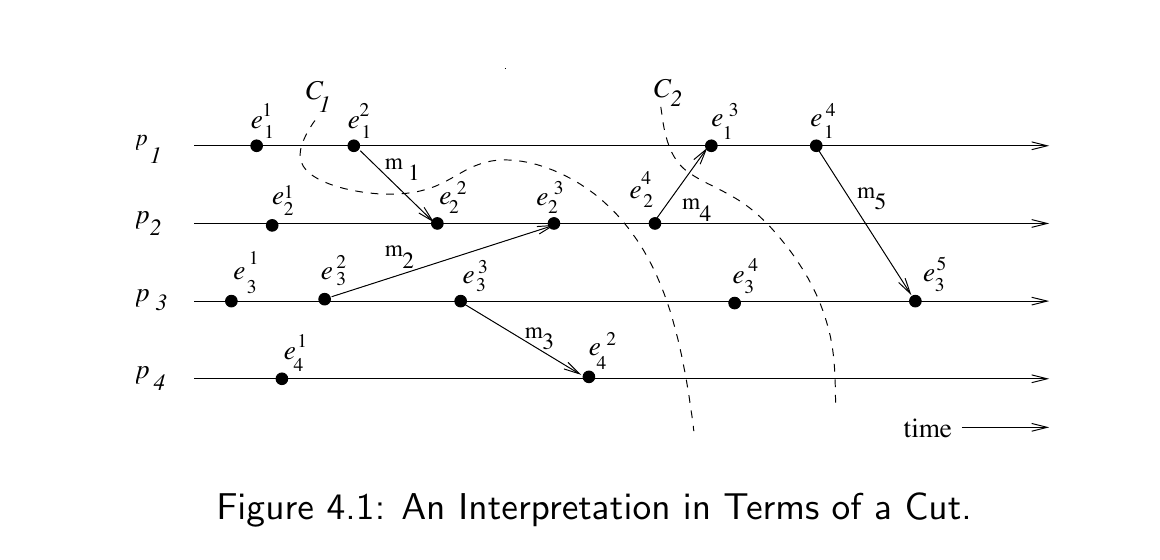
\includegraphics[width=.91\linewidth,height=.61\paperheight,keepaspectratio]{assets/week04-source-2025/cut-interpretation.png}
\end{center}
\smallnote{$C_1$ 有消息从未来流向过去；$C_2$ 是一致切面，穿越它的在途消息进入信道状态。}
\end{frame}

\begin{frame}{记录全局状态的两个问题}
\begin{enumerate}
  \item \key{I1：}哪些消息应纳入快照？
  \begin{itemize}
    \item 进程记录局部状态之前发送的消息必须被记录；
    \item 进程记录局部状态之后发送的消息不能被记录为快照中的在途消息。
  \end{itemize}
  \item \key{I2：}进程何时记录局部状态？
  \begin{itemize}
    \item 接收一个由远端快照之后发送的消息之前，必须先记录自己的状态；
    \item 否则会把结果纳入过去而遗漏其原因。
  \end{itemize}
\end{enumerate}
\end{frame}

\sectionframe{FIFO 信道上的 Chandy--Lamport}{用 marker 在每条 FIFO 信道上划出快照边界，既记录节点，也记录边界内的在途消息。}

\begin{frame}{Marker 的作用}
\begin{itemize}
  \item marker 是控制消息，不是应用消息；
  \item FIFO 保证 marker 之后发送的应用消息不会越过 marker 先到达；
  \item 因而 marker 将信道消息分为“快照前”和“快照后”；
  \item 进程记录局部状态后，必须先沿每条出信道发送 marker，再发送新的应用消息；
  \item 进程不晚于收到任意入信道 marker 时记录局部状态。
\end{itemize}
\end{frame}

\begin{frame}{Chandy--Lamport：发起规则}
任意进程都可以发起一次快照。发起者执行：
\begin{enumerate}
  \item 记录自己的局部状态；
  \item 对每条尚未发送 marker 的出信道发送 marker；
  \item 在 marker 之后才继续发送应用消息。
\end{enumerate}
\vfill
\callout{局部边界}{marker 发送顺序把“记录状态”和“之后的应用消息”分隔开。}
\end{frame}

\begin{frame}{Chandy--Lamport：接收规则}
进程 $p_j$ 收到信道 $C_{ij}$ 上的 marker：
\begin{itemize}
  \item 若尚未记录局部状态：记录 $LS_j$，把 $C_{ij}$ 状态记为空，并执行发起规则；
  \item 若已经记录局部状态：把该信道上自记录 $LS_j$ 后到收到 marker 前收到的应用消息记入 $SC_{ij}$；
  \item 当每条入信道都收到 marker，$p_j$ 的本地快照完成。
\end{itemize}
\end{frame}

\begin{frame}{算法伪代码：Marker Sending Rule}
\begin{block}{Marker Sending Rule for process $i$}
\begin{enumerate}
  \item $p_i$ 记录自己的状态；
  \item 对每条尚未发送 marker 的出信道 $C$，先发送 marker；
  \item 之后才允许沿 $C$ 发送新的应用消息。
\end{enumerate}
\end{block}
\vfill
\begin{block}{Marker Receiving Rule for process $j$}
收到 marker 后，若首次记录则把该信道记为空并执行 Sending Rule；否则记录该信道上 marker 前的消息。
\end{block}
\end{frame}

\begin{frame}{Chandy--Lamport 完整例子：Marker 如何传播}
\small
三进程通过 FIFO 信道通信；$p_1$ 发起快照。应用消息 $m$ 已由 $p_3$ 发往 $p_2$，但尚未到达。
\begin{center}
\begin{tabularx}{.96\linewidth}{>{\bfseries}p{1.2cm}>{\raggedright\arraybackslash}p{3cm}>{\raggedright\arraybackslash}X}
\toprule
时刻 & 事件 & 本地记录动作 \\
\midrule
$t_0$ & $p_3\rightarrow p_2:m$ & $m$ 在 $C_{32}$ 中延迟。 \\
$t_1$ & $p_1$ 发起快照 & 记录 $LS_1$，先向 $p_2,p_3$ 发送 Marker。 \\
$t_2$ & $p_2$ 首次收到 Marker & 记录 $LS_2$；$SC_{12}=\varnothing$；开始记录其他入信道。 \\
$t_3$ & $p_3$ 首次收到 Marker & 记录 $LS_3$；$SC_{13}=\varnothing$；向 $p_2$ 发送 Marker。 \\
$t_4$ & $p_2$ 收到应用消息 $m$ & 因 $C_{32}$ 的 Marker 尚未到达，把 $m$ 记入 $SC_{32}$。 \\
$t_5$ & $p_2$ 收到 $p_3$ 的 Marker & 关闭 $C_{32}$ 的记录，得到 $SC_{32}=\{m\}$。 \\
\bottomrule
\end{tabularx}
\end{center}
\smallnote{FIFO 保证 $p_3$ 在记录状态后发送的 Marker 不会越过更早发送的 $m$。}
\end{frame}

\begin{frame}{Chandy--Lamport 完整例子：最终快照如何组成}
\small
\begin{columns}[T,onlytextwidth]
\column{.45\textwidth}
\begin{block}{最终记录结果}
\[
\{LS_1@t_1,\ LS_2@t_2,\ LS_3@t_3\}
\]
\[
SC_{32}=\{m\},\qquad
SC_{ij}=\varnothing\ (ij\neq32).
\]
\end{block}
\column{.51\textwidth}
\begin{enumerate}
  \item $send(m)\in LS_3$：$p_3$ 在 $t_3$ 记录前已经发送 $m$；
  \item $recv(m)\notin LS_2$：$p_2$ 在 $t_2$ 记录后才收到 $m$；
  \item 因此 $m$ 必须且只应出现在信道状态 $SC_{32}$；
  \item 其他信道在记录区间内没有应用消息，状态为空。
\end{enumerate}
\end{columns}
\vfill
\callout{一致性检查}{快照没有“只记录接收、不记录发送”；跨越切面的唯一应用消息 $m$ 被准确保存为在途消息。}
\end{frame}

\begin{frame}{为什么 FIFO 保证信道状态正确}
对信道 $C_{ij}$：
\begin{itemize}
  \item $p_i$ 在记录状态后发送 marker；
  \item FIFO 保证 marker 之后发送的应用消息不能先于 marker 到达 $p_j$；
  \item 因而 $p_j$ 在收到 marker 前看到的消息，恰好是发送方状态之后且 marker 之前发送的消息；
  \item 这些消息已发送但尚未接收，正是 $SC_{ij}$。
\end{itemize}
\end{frame}

\begin{frame}{Chandy--Lamport 的正确性分解}
\begin{itemize}
  \item \key{C2：}marker 之后发送的消息不会被记录，因为 marker 先到；
  \item \key{C1：}若接收消息先于 marker 到达，则接收方在记录状态前纳入它；若晚于本地状态但早于 marker，则放入信道状态；
  \item 每个消息恰好落在发送方局部状态、接收方局部状态或信道状态中的一个位置；
  \item 由此得到一致全局状态。
\end{itemize}
\end{frame}

\begin{frame}{复杂度与终止}
对单次快照实例：
\begin{itemize}
  \item 记录阶段控制消息数为 $O(e)$，其中 $e$ 是网络边数；
  \item 时间复杂度为 $O(d)$，其中 $d$ 是网络直径；
  \item 进程在所有入信道收到 marker 后完成局部记录；
  \item 收集或传播局部快照可以通过额外树结构完成；
  \item 算法不要求暂停应用计算。
\end{itemize}
\end{frame}

\begin{frame}{记录快照未必是原执行中出现过的瞬时状态}
\begin{itemize}
  \item 不同进程可能在不同真实时刻记录局部状态；
  \item 所得组合未必等于原执行某一时刻的 $GS$；
  \item 但它是某个等价执行中的合法状态；
  \item 对稳定性质（成立后不会失效），若快照前已成立，则在记录快照中仍成立；
  \item 因此快照适合检测终止、死锁、稳定谓词和恢复点。
\end{itemize}
\end{frame}

\begin{frame}{课堂互动：追踪 marker 和在途消息}
\begin{columns}[T,onlytextwidth]
\column{.56\textwidth}
\begin{center}
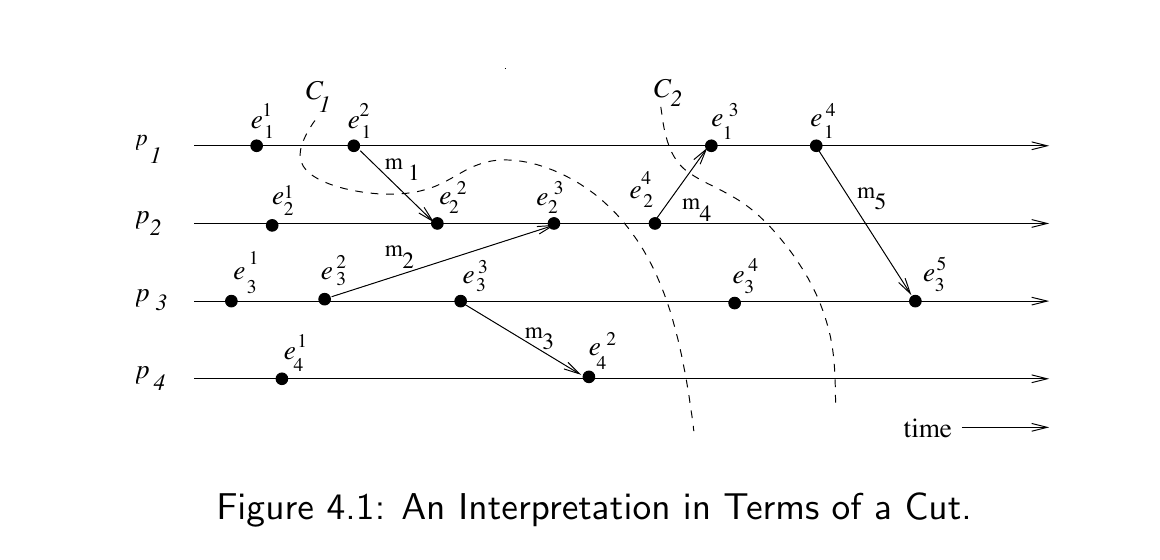
\includegraphics[width=\linewidth,height=.54\paperheight,keepaspectratio]{assets/week04-source-2025/cut-interpretation.png}
\end{center}
\column{.39\textwidth}
\begin{enumerate}
  \item 选择一个发起进程；
  \item 在每条信道标出 marker；
  \item 列出每个进程的局部状态记录时刻；
  \item 找出所有进入 $SC_{ij}$ 的消息；
  \item 判断最终 cut 是否一致。
\end{enumerate}
\end{columns}
\end{frame}

\sectionframe{并发发起与快照传播}{多个进程同时发起快照时，记录阶段可以共享控制消息；传播阶段需要识别区域和生成树。}

\begin{frame}{Spezialetti--Kearns：并发发起的现实问题}
\begin{itemize}
  \item 多个进程可能几乎同时启动快照；
  \item 每个 marker 携带发起者标识；
  \item 进程维护 $master$ 变量表示当前所属发起者/区域；
  \item 不同 $master$ 的 marker 表示跨区域边界；
  \item $id\text{-}border\text{-}set$ 保存邻居区域的发起者标识。
\end{itemize}
\end{frame}

\begin{frame}{区域与跨区域信道}
\begin{columns}[T,onlytextwidth]
\column{.47\textwidth}
\blocktitle{区域}
\begin{itemize}
  \item 所有 $master$ 相同的进程组成一个区域；
  \item 每个并发发起者隐式拥有一棵生成树；
  \item 首次 marker 的发送者成为树上的 parent。
\end{itemize}
\column{.47\textwidth}
\blocktitle{跨区域边界}
\begin{itemize}
  \item marker 来源的 $master$ 与本地不同；
  \item 发送者位于邻接区域；
  \item 信道状态仍按 Chandy--Lamport 规则记录；
  \item 边界关系用于后续合并和传播。
\end{itemize}
\end{columns}
\end{frame}

\begin{frame}{快照记录阶段：状态与信道照常记录}
\begin{itemize}
  \item 每个进程在每条入信道收到 marker 后完成本地快照；
  \item 跨区域信道也记录 marker 前的在途消息；
  \item 记录阶段结束后，系统被划分为与并发发起次数相等的区域；
  \item 每个区域的进程和信道构成该发起者的局部快照；
  \item 关键差异在于“谁负责收集和传播”，不是局部一致性规则。
\end{itemize}
\end{frame}

\begin{frame}{隐式生成树：让快照传播从全网广播变成聚合}
\begin{itemize}
  \item 发起者是生成树根；
  \item 进程第一次从 $p_j$ 收到 marker，则 $p_j$ 是自己的 parent；
  \item 其他发送 marker 的邻居被视为 child 或边界邻居；
  \item 中间进程等待所有 child 的记录后向 parent 聚合；
  \item 根收到全部后组装其区域的完整快照。
\end{itemize}
\end{frame}

\begin{frame}{区域快照的组装与跨区域交换}
\begin{enumerate}
  \item 每个进程向 parent 发送本地状态、入信道状态和子树结果；
  \item 发起者组装本区域内所有进程及关联信道；
  \item 相邻区域的发起者按轮次交换区域快照；
  \item 组合后可得到全系统快照或按区域查询；
  \item 记录阶段消息复杂度为 $O(e)$；组装/传播约为 $O(rn^2)$。
\end{enumerate}
\vfill
\smallnote{$r$ 为并发发起数，$n$ 为进程数，具体常数依赖拓扑。}
\end{frame}

\sectionframe{Non-FIFO 信道上的快照}{marker 可能被后发消息越过，必须把控制边界嵌入应用消息或显式追踪白色历史。}

\begin{frame}{为什么 FIFO marker 在 Non-FIFO 中失效}
\begin{itemize}
  \item Non-FIFO 信道像消息集合，接收方可任意取出消息；
  \item marker 发送后，后发的应用消息可能先抵达；
  \item 收到 marker 时无法仅凭队列位置判断哪些消息属于边界前；
  \item 算法必须增加抑制、着色、计数或 piggyback 控制信息；
  \item 目标仍是区分“发送方快照前发送”和“快照后发送”。
\end{itemize}
\end{frame}

\begin{frame}{Lai--Yang：用颜色代替 marker}
\begin{enumerate}
  \item 所有进程初始为白色；记录快照时变为红色，并执行等价的发送规则；
  \item 白进程发送白消息，红进程发送红消息；
  \item 白消息表示发送者记录快照之前发送，红消息表示之后发送；
  \item 白进程最迟在收到红消息时记录自身快照；
  \item 颜色随每条计算消息传播，不依赖 FIFO 交付。
\end{enumerate}
\end{frame}

\begin{frame}{Lai--Yang：白色消息历史}
白进程需要沿每条信道记录白消息的发送/接收历史：
\begin{itemize}
  \item 记录快照时，白消息历史成为局部快照的一部分；
  \item 进程转红后，把自身快照和这些历史发送给发起者；
  \item 发起者用发送集合减去接收集合计算信道状态；
  \item 该方法用消息历史换取对 Non-FIFO 乱序的鲁棒性。
\end{itemize}
\end{frame}

\begin{frame}{Lai--Yang 的信道状态公式}
对信道 $C_{ij}$：
\[
SC_{ij}
=\{send(m_{ij})\mid send(m_{ij})\in LS_i\}
-\{rec(m_{ij})\mid rec(m_{ij})\in LS_j\}.
\]
\begin{itemize}
  \item 只考虑白消息历史；
  \item 发送方状态中的白消息已经发生；
  \item 接收方状态中尚未出现的白消息仍在途；
  \item 红消息不属于本次快照的信道状态。
\end{itemize}
\end{frame}

\begin{frame}{Mattern：用向量时间选定快照边界}
以下是 Mattern 思路的教学化版本（完整协议还需明确白/红消息、终止证据和计数器初始化），基于向量时钟并假设单一发起者：
\begin{enumerate}
  \item 发起者选择未来向量时间 $s$，广播该值并等待所有确认；
  \item 每个进程收到后记住 $s$ 并返回确认；
  \item 发起者把自己的向量时钟推进到 $s$，广播 dummy 消息；
  \item dummy 消息迫使接收方把时钟推进到至少 $s$；
  \item 进程在时钟从 $<s$ 变为 $\ge s$ 前记录局部状态并发送给发起者。
\end{enumerate}
\end{frame}

\begin{frame}{Mattern：按向量时间计算信道状态}
信道 $C_{ij}$ 的状态为：
\begin{itemize}
  \item 在发送方向量时间戳小于 $s$ 的消息；
  \item 但这些消息在接收方记录 $LS_j$ 后才被收到；
  \item 向量时钟把控制消息与应用消息的因果关系统一起来；
  \item 关键优势是不需要保存完整消息历史；
  \item 关键代价是需要终止检测，确认没有白消息仍在途。
\end{itemize}
\end{frame}

\begin{frame}{Mattern 的 Non-FIFO 终止检测：计数法}
每个进程维护：
\[
cntr_i=\#\text{快照前发送的白消息}-\#\text{快照前收到的白消息}.
\]
\begin{itemize}
  \item 进程将 $cntr_i$ 与局部快照报告给发起者；
  \item 快照后收到的白消息转发给发起者；
  \item 发起者收到总数为 $\sum_i cntr_i$ 的转发白消息后，确认没有白消息在途；
  \item 计数的正负平衡提供全局终止证据。
\end{itemize}
\end{frame}

\begin{frame}{Mattern 的终止检测：逐信道 piggyback}
第二种方法：
\begin{itemize}
  \item 每条红消息携带该信道在本地快照前发送的白消息数；
  \item 接收方维护每条信道收到的白消息计数；
  \item 当实际收到的白消息数达到红消息携带值，认为该入信道记录完成；
  \item 不必把白消息全部转发给中心；
  \item 需要额外计数器和控制字段。
\end{itemize}
\end{frame}

\sectionframe{因果消息交付下的快照}{因果有序信道让控制 token 自带边界语义，算法可减少消息历史和全局协调。}

\begin{frame}{Causal delivery 提供内置同步}
因果消息交付满足：
\[
send(m_{ij})\rightarrow send(m_{kj})
\Rightarrow
rec(m_{ij})\rightarrow rec(m_{kj}).
\]
\begin{itemize}
  \item 控制 token 的因果位置可以约束后续应用消息；
  \item Acharya--Badrinath 与 Alagar--Venkatesan 都以此为基础；
  \item 两者记录进程状态的方式相同；
  \item 差异主要在信道状态的计算与终止方式。
\end{itemize}
\end{frame}

\begin{frame}{Causal snapshot 的共同状态记录步骤}
\begin{enumerate}
  \item 发起者向所有进程（包括自己）广播 token；
  \item 进程 $p_i$ 收到 $token_i$ 时记录 $LS_i$；
  \item $p_i$ 把局部快照发送给发起者；
  \item 发起者收齐所有局部快照后，算法的进程状态记录阶段结束；
  \item 信道状态按具体算法的计数或旧消息定义恢复。
\end{enumerate}
\end{frame}

\begin{frame}{正确性：为什么未记录发送不会出现已记录接收}
若 $send(m_{ij})\notin LS_i$，假设反之 $rec(m_{ij})\in LS_j$：
\begin{itemize}
  \item token 的接收在各进程局部状态记录之前建立因果边界；
  \item 因果交付会把 token 的因果后继排在消息接收之前；
  \item 因而 $rec(m_{ij})$ 不可能已经位于 $LS_j$；
  \item 得到矛盾，说明由 token 得到的局部状态组合满足一致性。
\end{itemize}
\end{frame}

\begin{frame}{Acharya--Badrinath：发送/接收计数数组}
每个进程 $p_i$ 维护：
\[
SENT_i[1..N],\qquad RECD_i[1..N].
\]
其中：
\begin{itemize}
  \item $SENT_i[j]$：$p_i$ 向 $p_j$ 发送的消息数；
  \item $RECD_i[j]$：$p_i$ 从 $p_j$ 接收的消息数；
  \item 记录 $LS_i$ 时，把两个数组一并保存；
  \item 发起者根据发送与接收序号差计算每条信道上的在途消息范围。
\end{itemize}
\end{frame}

\begin{frame}{Acharya--Badrinath：信道状态与复杂度}
对从 $p_i$ 到 $p_j$ 的信道：
\[
SC_{ij}=\{RECD_j[i]+1,\ldots,SENT_i[j]\}.
\]
\begin{itemize}
  \item 发起者到各进程的信道可直接视为空；
  \item 消息序号区间直接给出在途集合；
  \item 在完全互连、可靠因果交付且采用本页中心化收集的简化模型下，记录与组装约需 $2n$ 条消息和 2 个消息传输时间单位；
  \item 若需要消息内容，还需额外传送内容。
\end{itemize}
\end{frame}

\begin{frame}{Alagar--Venkatesan：old 与 new 消息}
定义：
\begin{itemize}
  \item 若消息的发送因果先于 token 的发送，称为 old；
  \item 否则称为 new；
  \item 进程收到 token 时记录局部状态，并将所有信道状态初始化为空；
  \item 此后只有收到的 old 消息才加入相应信道状态；
  \item 发起者收齐 Done 后广播 Terminate，所有进程停止该快照实例。
\end{itemize}
\end{frame}

\begin{frame}{算法特征对照}
\begin{tabularx}{\linewidth}{>{\bfseries}p{2.8cm}XX}
\toprule
算法 & 假设/核心机制 & 主要代价或特点 \\
\midrule
Chandy--Lamport & FIFO marker & $O(e)$ 消息，$O(d)$ 时间 \\
Spezialetti--Kearns & 并发发起、区域生成树 & 记录 $O(e)$，组装约 $O(rn^2)$ \\
Lai--Yang & Non-FIFO 颜色与历史 & 需要消息历史 \\
Mattern & 向量时间与终止检测 & 不需完整历史，需白消息终止证据 \\
Acharya--Badrinath & 因果交付、计数数组 & 约 $2n$ 消息、中心化信道计算 \\
Alagar--Venkatesan & 因果交付、old 消息 & 约 $3n$ 消息、分布式信道计算 \\
\bottomrule
\end{tabularx}
\end{frame}

\sectionframe{一致快照的检查点理论}{局部检查点异步产生；zigzag path 比因果路径更精确地刻画“能否共同出现在某个一致快照”。}

\begin{frame}{局部检查点与检查点区间}
\begin{itemize}
  \item 进程运行中周期性保存局部状态，称为 local checkpoint；
  \item $p_q$ 的第 $i$ 个检查点记为 $C_{q,i}$；
  \item 每个进程在执行开始前有初始检查点，结束后有虚拟检查点；
  \item 第 $i$ 个检查点区间包含从 $C_{q,i-1}$ 之后到 $C_{q,i}$ 之前的计算；
  \item 一致快照是每个进程选择一个检查点，且它们可以共同形成因果一致切面。
\end{itemize}
\end{frame}

\begin{frame}{没有因果路径也不一定能组成一致快照}
在某些执行中，$C_{1,1}$ 与 $C_{3,2}$ 互不发生在先，但仍不能与任意 $p_2$ 检查点组合成一致快照。
\vfill
\begin{itemize}
  \item 单纯检查 happened-before 不够；
  \item 消息可能在前一条消息被接收之前就从另一个检查点区间发出；
  \item 这种“跨区间消息链”会限制可选的局部检查点；
  \item Netzer--Xu 用 zigzag path 捕获这种约束。
\end{itemize}
\end{frame}

\begin{frame}{Figure 4.2：检查点与 zigzag path}
\begin{center}
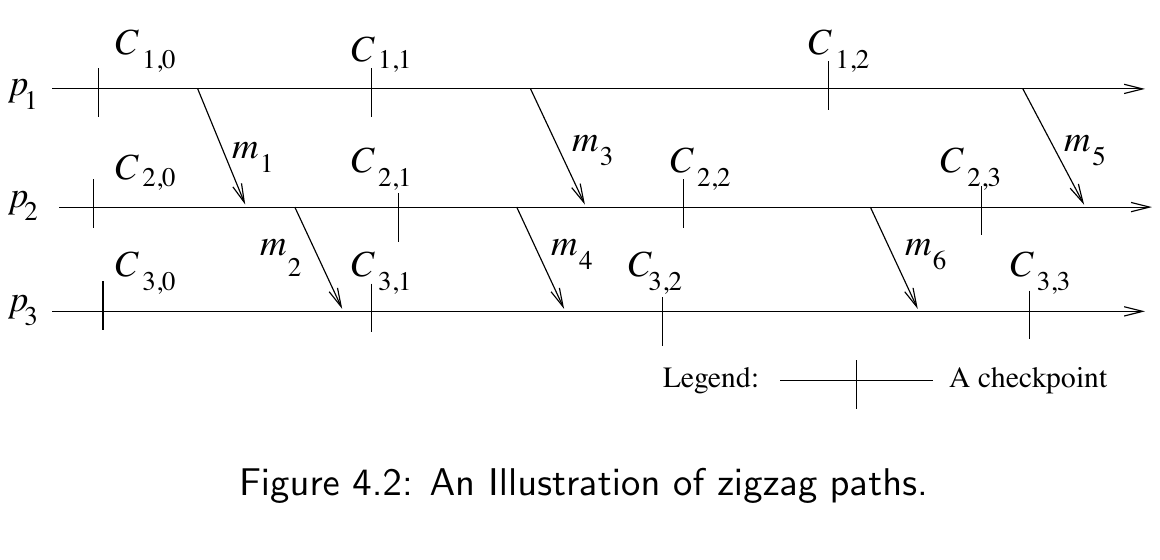
\includegraphics[width=.92\linewidth,height=.61\paperheight,keepaspectratio]{assets/week04-source-2025/checkpoint-order.png}
\end{center}
\smallnote{图中消息链可在前一消息接收前就发送下一消息，因此未必形成普通因果路径。}
\end{frame}

\begin{frame}{Zigzag path 的定义}
从检查点 $C_{x,i}$ 到 $C_{y,j}$ 存在 zigzag path，当且仅当存在消息 $m_1,\ldots,m_n$：
\begin{enumerate}
  \item $m_1$ 由 $p_x$ 在 $C_{x,i}$ 之后发送；
  \item 若 $m_k$ 被 $p_z$ 接收，则 $m_{k+1}$ 由 $p_z$ 在同一或更晚检查点区间发送；发送可以早于或晚于 $m_k$ 的接收；
  \item $m_n$ 在 $C_{y,j}$ 之前被 $p_y$ 接收。
\end{enumerate}
\end{frame}

\begin{frame}{Zigzag path 与因果路径的区别}
\begin{tabularx}{\linewidth}{>{\bfseries}p{2.9cm}XX}
\toprule
 & 因果路径 & Zigzag path \\
\midrule
消息链 & 后一消息在前一消息接收后发送 & 后一消息可在前一消息接收前发送 \\
范围 & 一定是 zigzag path & 不一定是因果路径 \\
是否可能成环 & 不能形成因果环 & 可以形成 zigzag cycle \\
用途 & 证明直接因果依赖 & 判定检查点能否共同出现 \\
\bottomrule
\end{tabularx}
\vfill
\callout{关系}{因果路径是 zigzag path 的特殊情况；zigzag 约束更强地刻画一致快照可扩展性。}
\end{frame}

\begin{frame}{Zigzag cycle：一个检查点无法进入一致快照}
若存在从检查点 $C$ 回到自身的 zigzag path，则称 $C$ 处于 zigzag cycle：
\begin{itemize}
  \item 选择 $C$ 会迫使某个检查点在其自身之前；
  \item 因此不存在包含 $C$ 的一致全局快照；
  \item Figure 4.3 中 $C_{2,1}$ 被消息 $m_1,m_2$ 组成的 Z-cycle 围住；
  \item 检测 Z-cycle 是检查点筛选的第一步。
\end{itemize}
\end{frame}

\begin{frame}{Figure 4.3：Zigzag cycle 与一致/不一致快照}
\begin{center}
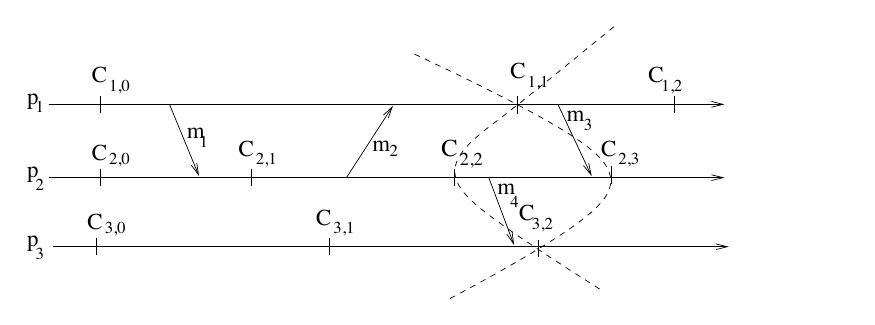
\includegraphics[width=.92\linewidth,height=.61\paperheight,keepaspectratio]{assets/week04-source-2025/zigzag-cycle-full.png}
\end{center}
\smallnote{$C_{2,1}$ 位于 Z-cycle 中；另一个切面可以避开该循环而保持一致。}
\end{frame}

\begin{frame}{一致快照的充要条件}
Netzer--Xu 定理：对检查点集合 $S$，存在包含 $S$ 的一致快照，当且仅当：
\[
\text{任意两个 }S\text{ 中检查点之间不存在 zigzag path}.
\]
推论：
\begin{itemize}
  \item 检查点 $C$ 能进入某个一致快照，当且仅当它不在 Z-cycle 中；
  \item 检查点集合若包含所有进程各一个点，并且集合内无 Z-path，则本身就是一致快照；
  \item “无因果路径”只是必要条件，不是充要条件。
\end{itemize}
\end{frame}

\begin{frame}{Z-cone 与 C-cone}
对检查点集合 $S$：
\begin{itemize}
  \item Z-cone：与 $S$ 之间既无 Z-path 到达，也无 Z-path 离开的检查点集合；
  \item C-cone：与 $S$ 之间既无普通因果路径到达，也无普通因果路径离开的集合；
  \item 因为因果路径一定是 Z-path，所以 $Z\text{-cone}\subseteq C\text{-cone}$；
  \item 真正可用于构造一致快照的候选点必须落在 Z-cone 中。
\end{itemize}
\end{frame}

\begin{frame}{Z-cone：可与检查点集合 $S$ 共同出现的候选区}
\begin{center}
\begin{tikzpicture}[font=\small,>=Latex,scale=.88,transform shape]
  \node[draw=ADSBlue,fill=ADSLightBlue,rounded corners,minimum width=2.2cm,minimum height=.85cm] (S) at (0,-.15) {检查点集合 $S$};
  \fill[ADSOrange!10] (-6,-2.2) rectangle (-2.0,2.2);
  \fill[ADSGreen!10] (-2.0,-2.2) rectangle (2.0,2.2);
  \fill[ADSBlue!8] (2.0,-2.2) rectangle (6,2.2);
  \draw[ADSGray] (-2,-2.2)--(-2,2.2);\draw[ADSGray] (2,-2.2)--(2,2.2);
  \node[text=ADSOrange,align=center,font=\bfseries] at (-4,1.55) {能通过 Z-path\\到达 $S$};
  \node[text=ADSGreen,align=center,font=\bfseries] at (0,1.55) {Z-cone\\与 $S$ Z-无序};
  \node[text=ADSBlue,align=center,font=\bfseries] at (4,1.55) {$S$ 能通过 Z-path\\到达};
  \node[draw=ADSOrange!70!black,fill=ADSOrange!10,rounded corners=2pt,minimum width=1.6cm,minimum height=.62cm,align=center,font=\scriptsize]
    (a) at (-4,-.4) {候选点 $a$};
  \node[draw=ADSGreen!70!black,fill=ADSGreen!10,rounded corners=2pt,minimum width=1.6cm,minimum height=.62cm,align=center,font=\scriptsize]
    (b) at (0,-1.45) {候选点 $b$};
  \node[draw=ADSBlue!70!black,fill=ADSBlue!10,rounded corners=2pt,minimum width=1.6cm,minimum height=.62cm,align=center,font=\scriptsize]
    (c) at (4,-.4) {候选点 $c$};
  \draw[\arrow,ADSOrange] (a)--(S);\draw[\arrow,ADSBlue] (S)--(c);
  \draw[ADSGreen,dashed] (b)--node[right,font=\scriptsize]{无 Z-path}(S);
\end{tikzpicture}
\end{center}
\smallnote{只有中间区域满足“既不能通过 Z-path 到达 $S$，也不能被 $S$ 通过 Z-path 到达”；这比普通因果并发更严格。}
\end{frame}

\begin{frame}{候选点仍需排除自身 Z-cycle}
即使检查点位于 $S$ 的 Z-cone，也可能无法加入：
\begin{itemize}
  \item 它自身处于 Z-cycle；
  \item 或与已经选择的其他候选点之间存在 Z-path；
  \item 因此先按每个进程构造 $S_{useful}^q$：与 $S$ 互相无 Z-path，且自身无 Z-cycle；
  \item 再从不同进程的 useful 集合中选择彼此无 Z-path 的组合。
\end{itemize}
\end{frame}

\begin{frame}{Lemma 4.1：单个候选点的可扩展性}
设 $S$ 中无 Z-path，$C_{q,i}\notin S$。则：
\[
S\cup\{C_{q,i}\}\text{ 可扩展为一致快照}
\Longleftrightarrow
C_{q,i}\in S_{useful}^q.
\]
\begin{itemize}
  \item useful 条件排除与 $S$ 的 Z-path 冲突；
  \item 同时排除候选点自身的 Z-cycle；
  \item 该引理把全局搜索缩小为每个进程的候选集合。
\end{itemize}
\end{frame}

\begin{frame}{Theorem 4.2：从候选集合选择完整快照}
设 $S\cap T=\varnothing$。$S\cup T$ 是一致全局快照，当且仅当：
\begin{enumerate}
  \item $T\subseteq S_{useful}$；
  \item $T$ 内部不存在 Z-path，即 $T\not\leadsto T$；
  \item $|S\cup T|=N$，每个进程恰好选择一个检查点。
\end{enumerate}
\vfill
\callout{组合约束}{合法候选点不等于合法组合；最后仍需检查候选点之间的相互关系。}
\end{frame}

\begin{frame}{Manivannan--Netzer--Singhal 枚举算法}
\begin{enumerate}
  \item 若输入集合 $S$ 已包含 Z-path 冲突，返回空；
  \item 找出尚未被 $S$ 表示的进程集合；
  \item 选一个未表示进程 $p_q$；
  \item 遍历 $S_{useful}^q$ 中的每个检查点，递归加入候选；
  \item 当所有进程都被表示时，将当前集合加入结果 $G$。
\end{enumerate}
\vfill
\smallnote{算法显式计算包含给定 $S$ 的全部一致快照，而不仅仅找一个。}
\end{frame}

\begin{frame}{枚举算法：完整中文伪代码}
\scriptsize
\begin{columns}[T,onlytextwidth]
\column{.47\textwidth}
\begin{block}{主过程 $ComputeAllCgs(S)$}
1. $G\leftarrow\varnothing$；\\
2. 若 $S\not\leadsto S$：\\
\quad $AllProcs\leftarrow$ 尚未在 $S$ 中出现的进程；\\
\quad 调用 $ComputeAllCgsFrom(S,AllProcs)$；\\
3. 返回 $G$。
\end{block}
\column{.49\textwidth}
\begin{block}{递归过程 $ComputeAllCgsFrom(T,ProcSet)$}
1. 若 $ProcSet=\varnothing$：\\
\quad $G\leftarrow G\cup\{T\}$，返回；\\
2. 从 $ProcSet$ 任选进程 $p_q$；\\
3. 对每个 $C\in T_{useful}^{q}$：\\
\quad 调用 $ComputeAllCgsFrom($\\
\qquad $T\cup\{C\},ProcSet\setminus\{p_q\})$。
\end{block}
\end{columns}
\normalsize
\vfill
\callout{变量含义}{$T$ 是当前已选择的检查点集合；$T_{useful}^{q}$ 只保留与 $T$ 无 Z-path 冲突且自身不在 Z-cycle 中的 $p_q$ 检查点。}
\end{frame}

\begin{frame}{枚举算法例子：为什么要回溯？}
\small
已有 $S=\{C_{1,2}\}$，还需从 $p_2,p_3$ 各选择一个检查点：
\begin{center}
\begin{tabularx}{.94\linewidth}{>{\bfseries}p{2.2cm}X X}
\toprule
递归层 & 候选集合 & 动作与结果 \\
\midrule
$p_2$ & $S_{useful}^{2}=\{C_{2,1},C_{2,3}\}$ & 分成两个搜索分支 \\
$p_3$（分支 A） & $\{C_{3,2}\}$ & 若与 $C_{2,1}$ 无 Z-path，得到一个一致快照 \\
$p_3$（分支 B） & $\{C_{3,1},C_{3,4}\}$ & 逐个检查与 $C_{2,3}$ 的 Z-path；冲突分支剪枝 \\
结束 & 每个进程恰有一个检查点 & 把所有合法集合加入 $G$ \\
\bottomrule
\end{tabularx}
\end{center}
\begin{itemize}
  \item useful 是相对于“当前集合 $T$”计算的；加入一个检查点后，后续候选可能改变。
  \item 因此算法不能先为每个进程独立选点再拼接，而要边选择、边检查、边回溯。
\end{itemize}
\end{frame}

\begin{frame}{枚举算法的正确性与代价}
\begin{itemize}
  \item 搜索始终限制在 $S$ 的 Z-cone；
  \item 每次加入候选前检查 Z-cycle 与集合间 Z-path；
  \item 返回集合 $G$ 恰好包含所有包含 $S$ 的一致快照；
  \item 一致快照数量本身可能指数增长，因此枚举问题最坏情况下不可避免地昂贵；
  \item 实际系统通常使用剪枝、采样或只寻找满足目标性质的一个快照。
\end{itemize}
\end{frame}

\sectionframe{R-graph：把 Z-path 检查转成图搜索}{在已停止或已终止的执行中，用 rollback-dependency graph 表示检查点间的依赖。}

\begin{frame}{Rollback-dependency graph 的定义}
R-graph 是有向图 $G=(V,E)$：
\begin{itemize}
  \item 顶点 $V$ 是所有进程的检查点；
  \item 同一进程的连续检查点有边 $C_{p,i}\to C_{p,i+1}$；
  \item 若消息从 $p$ 的第 $i$ 个检查点区间发送，在 $q$ 的第 $j$ 个区间接收，则有边 $C_{p,i}\to C_{q,j}$；
  \item 终止前最后状态可表示为 volatile checkpoint。
\end{itemize}
\end{frame}

\begin{frame}{Figure 4.5：分布式执行与检查点}
\begin{center}
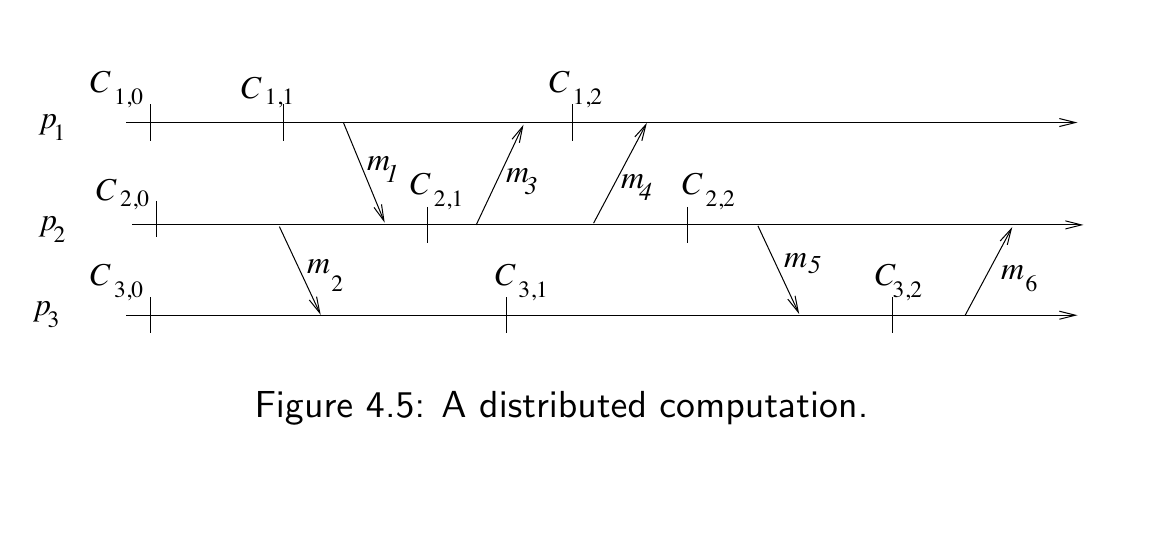
\includegraphics[width=.91\linewidth,height=.61\paperheight,keepaspectratio]{assets/week04-source-2025/distributed-computation-checkpoints.png}
\end{center}
\smallnote{每条进程线的检查点区间与跨进程消息共同决定 R-graph 边。}
\end{frame}

\begin{frame}{Figure 4.6：对应的 R-graph}
\begin{center}
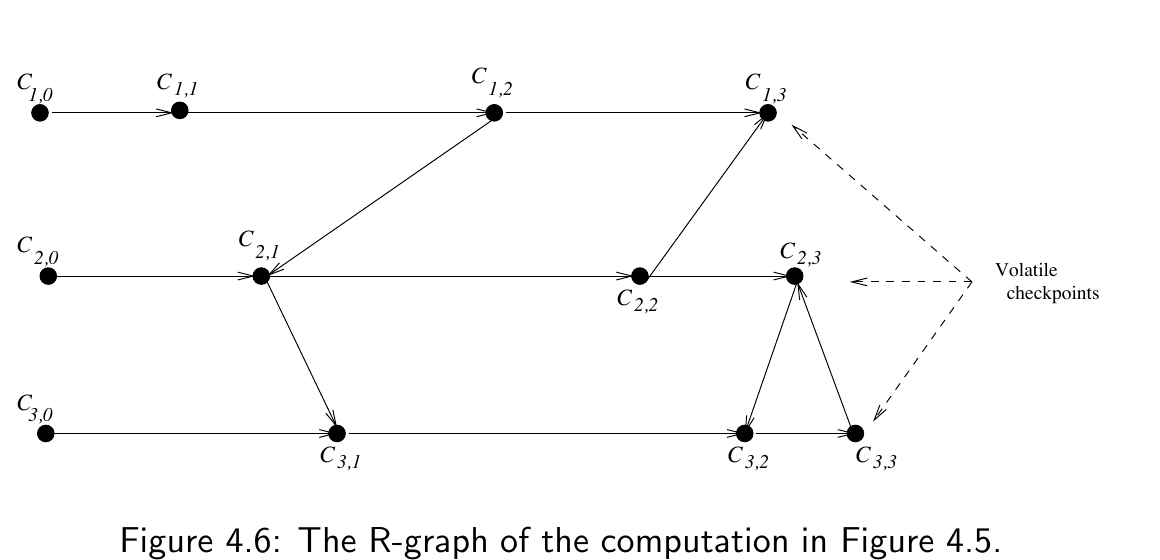
\includegraphics[width=.86\linewidth,height=.61\paperheight,keepaspectratio]{assets/week04-source-2025/r-graph.png}
\end{center}
\smallnote{虚线箭头表示 volatile checkpoint 相关的依赖；实线表示连续检查点或消息区间依赖。}
\end{frame}

\begin{frame}{R-graph 路径与 Z-path 的对应定理}
对检查点 $C_{p,i}$、$C_{q,j}$：存在从前者到后者的 Z-path，当且仅当：
\begin{enumerate}
  \item $p=q$ 且 $i<j$；或
  \item R-graph 中存在从 $C_{p,i+1}$ 到 $C_{q,j}$ 的有向路径。
\end{enumerate}
\vfill
\callout{算法意义}{在执行停止后，可用普通图搜索检测 Z-path，而不必重新播放所有消息。}
\end{frame}

\begin{frame}{R-graph 示例：从图路径读出 Z-path}
\begin{itemize}
  \item Figure 4.5 中从 $C_{1,1}$ 到 $C_{3,1}$ 存在 Z-path；
  \item 在 R-graph 中，对应为从 $C_{1,2}$ 到 $C_{3,1}$ 的路径；
  \item $C_{2,1}$ 位于 Z-cycle，因为 $C_{2,2}$ 可沿 R-graph 路径返回 $C_{2,1}$；
  \item 因此 $C_{2,1}$ 不能成为任何一致快照成员。
\end{itemize}
\end{frame}

\begin{frame}{课堂互动：检查点选择题}
给定三个进程及多个检查点：
\begin{enumerate}
  \item 标出每条跨进程消息所属检查点区间；
  \item 构造 R-graph；
  \item 判断指定检查点是否有 Z-path；
  \item 找出 Z-cycle；
  \item 枚举至少一个包含给定 $S$ 的一致快照；
  \item 说明为什么普通 causal path 检查会漏掉某个冲突。
\end{enumerate}
\end{frame}

\begin{frame}{AI 基础设施中的分布式快照}
\begin{itemize}
  \item GPU 训练 checkpoint 不仅是模型文件，还要包含 optimizer、数据迭代器和 in-flight collective 状态；
  \item 参数服务器/AllReduce 的消息在途状态决定恢复后是否重复应用更新；
  \item Ray、Kubernetes 控制器和数据流系统需要区分稳定事实与瞬时观测；
  \item 分布式 tracing 可把 marker 语义映射为 snapshot epoch 或 barrier token；
  \item 只要目标性质稳定，快照可用于检测“所有 worker 已停止”或“无未完成任务”。
\end{itemize}
\end{frame}

\begin{frame}{本讲总结}
\begin{itemize}
  \item 全局状态必须包含局部状态与信道状态；
  \item 一致 cut 不允许结果在过去、原因在未来；
  \item Chandy--Lamport 用 FIFO marker 构造一致快照；
  \item Non-FIFO 需要颜色、计数或向量时间；
  \item 因果交付让 token 自带边界语义；
  \item zigzag path/cycle 给出检查点一致性的充要条件；
  \item R-graph 把 Z-path 检查转化为有向图可达性。
\end{itemize}
\end{frame}

\begin{frame}{课堂互动：为真实系统写一个快照合同}
选择 Ray 训练、Kafka 流、Kubernetes 控制器或微服务请求链，写清：
\begin{enumerate}
  \item 进程、信道、局部状态和信道状态；
  \item FIFO、Non-FIFO 还是因果交付；
  \item marker、颜色、向量时间或计数器如何界定边界；
  \item 要检测的稳定谓词；
  \item 一个会使快照不一致的反例。
\end{enumerate}
\end{frame}

\begin{frame}[plain]
\begin{tikzpicture}[remember picture,overlay]
  \fill[ADSBlue] (current page.north west) rectangle (current page.south east);
  \fill[ADSOrange] (current page.south west) rectangle ([yshift=2mm]current page.south east);
  \node[align=center] at (current page.center) {\fontsize{38}{45}\selectfont\color{white}\bfseries 谢谢\\[5mm]
  \large\color{white!80}下一讲：分布式算法与消息传播};
\end{tikzpicture}
\end{frame}

\end{document}
